\section{Results}
If not stated differently the simulations use parameters as given in the table below:
\begin{table}[H]
    \centering
    \begin{tabular}{r|l}
        $N$ & $10^{5}$\\
        $D$ & $0,02$\\
        $R_s$ & $1$ \\
        $R_d$ & $10$ \\
        ${\rm d}t$ & $10^{-3}$
    \end{tabular}
    \caption{Default simulation parameters}
    \label{tab:Parameters}
\end{table}

\subsection{Ideal Sink without Potential Barrier}
The following figures show results of simulations using the model explained before. First we examine the dependence of the reaction rate on the diffusion constant. Therefore the simulation results are compared to the steady state analytic solution as given in \eqref{normalization}:
\begin{align}
    K &= 4 \pi R_s D \rho_o \\
    \rho_o &= N \left\{ \int_{R_s}^{R_d} \left( 1 - \frac{R_s}{r} \right) {\rm d} r \right\}^{-1}
    \label{Steady_state_rate}
\end{align}
\subsubsection{Varying Diffusion Coefficient$D$}
\begin{figure}[H]
    \centering
    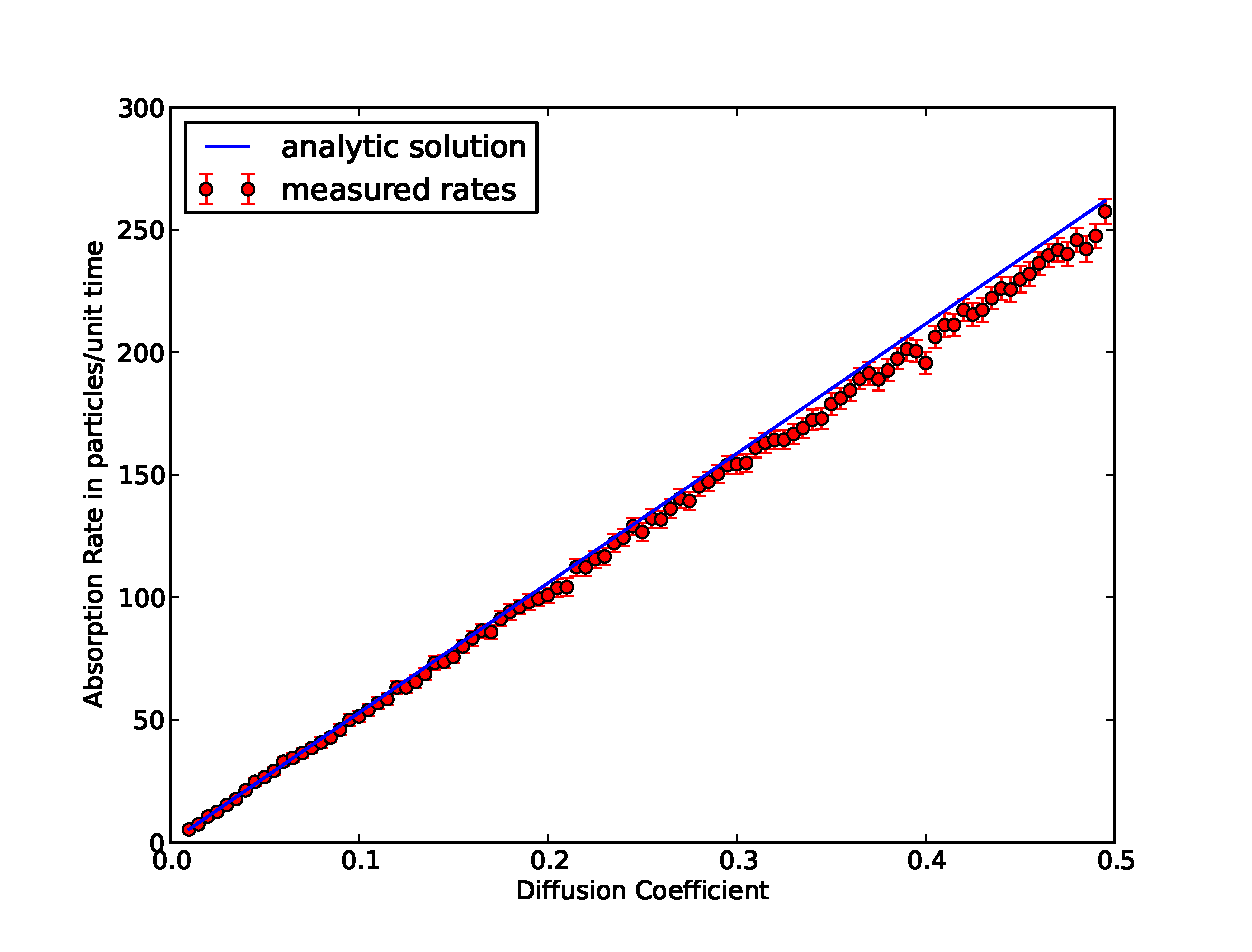
\includegraphics[width=.7 \textwidth, keepaspectratio]{plots/np/d/Kabs.eps}
    \caption{Reaction rates vs. Diffusion coefficient - Analytic solution and measured results}
    \label{fig:Kabs_D}
\end{figure}
The preceeding figure shows the results for several simulation runs with different diffusion coefficient. It is obvious that the simulation results show the correct linear behaviour for the reaction rate but have a systematic error of about $5 - 10 \%$. To give a better impression of the relational dependence the following plot shows relative quantities for the results:
\begin{figure}[H]
    \centering
    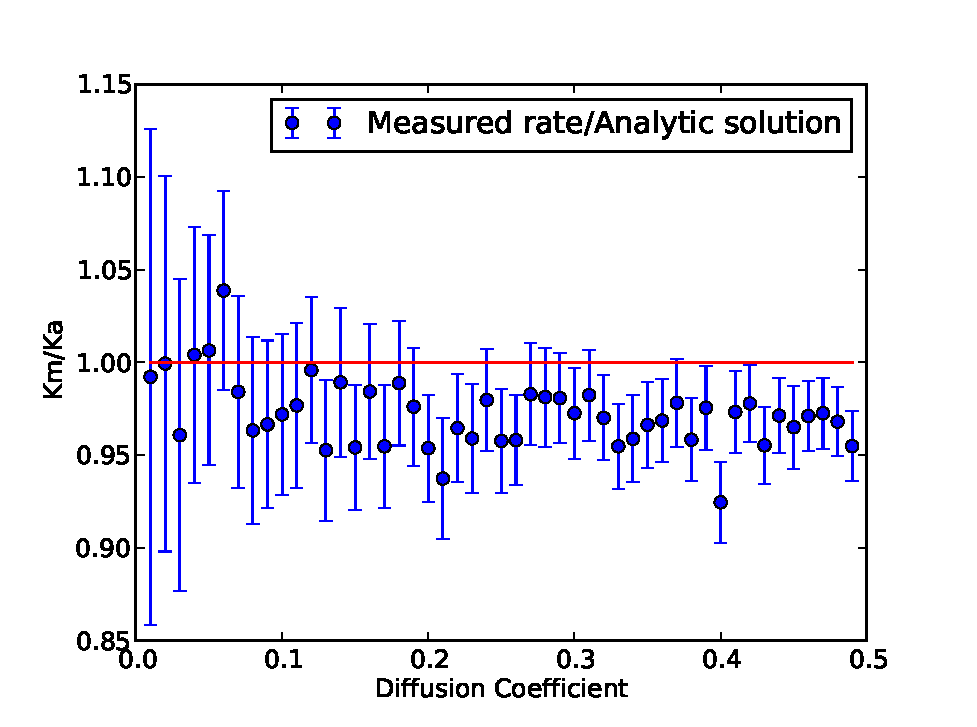
\includegraphics[width = .7 \textwidth, keepaspectratio]{plots/np/d/Krel.eps}
    \caption{Relative quantities for Reaction rates}
    \label{fig:Krel_d}
\end{figure}
For $D > 0.1$ the figure shows a systematic error of about $5 \%$ in the results for the reaction rates. For $D<0.1$ the results are distributed around the analytic solution, but mostly not within the error bars, that are at one $\sigma$. So there might be a flaw in the error calculation.

\subsubsection{Varying Sink Radius $R_s$}
This section gives results for different sink radius $R_s$ @ constant density $\rho_o$ to test the obvious linear relationship given in \eqref{Steady_state_rate}.
\begin{figure}[H]
    \centering
    \includegraphics[width = .7 \textwidth]{plots/np/rs/KabsRs.eps}
    \caption{Reaction rate vs. Sink Radius}
    \label{fig:KabsRs}
\end{figure}
The results presented in the figure above do qualitatively support the linear relation between sink radius and reaction rate.
The following figure strongly suggests, that the sumulation also quantitatively maps on the analytic solution.
\begin{figure}[H]
    \centering
    \includegraphics[width = .7 \textwidth]{plots/np/rs/KrelRs.eps}
    \caption{Normalized reaction rate vs. sink radius}
    \label{fig:KrelRs}
\end{figure}
The following figures present the obtained density profiles from the simulation.
\begin{figure}[H]
    \centering
    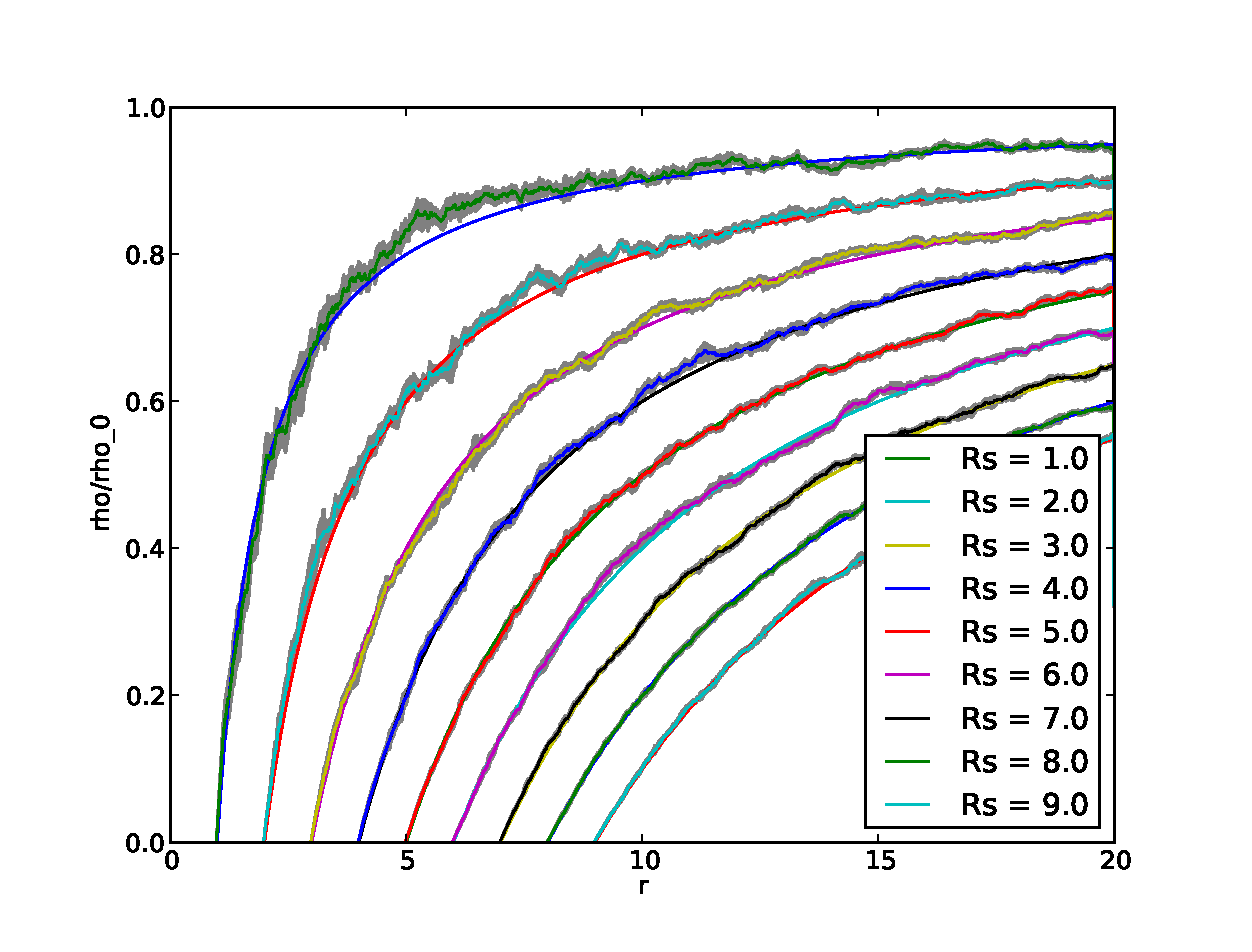
\includegraphics[width = .7 \textwidth]{plots/np/rs/rho_over_rho0.eps} 
    \caption{Normalized density profiles for different sink radius}
    \label{fig:ror0Rs}
\end{figure}
\subsubsection{Finite size analysis - Varying Domain Radius $R_d$}
This section shows plots for different domain radius $R_d$ @ constant density $\rho_o$.
This will point out finite size effects in the simulation (if they exist). 

